\documentclass[12pt]{report}
\usepackage{graphicx}

\title{Jr Penetration Tester}
\author{Emilio Junoy de Juambelz}
\date{\today}

\begin{document}

\chapter{Network security}

\section{Protocols and servers}

\subsection{Telnet}
El protocolo Telnet es un protocolo de la capa de aplicación
usado para conectarse a una terminal virtual u otra computadora.
Usando Telnet, un usuario puede conectarse a otra computadora y 
acceder a su terminal (console) para correr programas, empezar
procesos y realizar tareas del administrador de forma remota.\\

El protocolo Telnet es relativamente sencillo. Cuando un usario 
se conecta, se le pregunta por un nombre de usuario y una 
contraseña. Una vez que el usuario fue autorizado, tendrá acceso
a una terminal remota del sistema. Desafortunadamente, toda esta 
comunicación entre el cliente Telnet y el servidor Telnet no
está encriptada, lo que lo hace un objetivo fácil par los hackers.\\

Un servidor Telnet usa el protocolo Telnet para escuchar conexiones
entrantes en el puerto 23. Consideremos un ejemplo:\\
Un usuario se está conectando a $\textit{telnetd}$, un servidor
Telnet. Los pasos son como siguen:
\begin{enumerate}
  \item Primero, se le pide un nombre de usuario.
  \item Después, se le pide la contraseña (no se muestra).
  \item Una vez que inicia sesión es bienvenido con un mensaje.
  \item El servidor le da una terminal. El "\$" indica que no es
    una terminal root.
\end{enumerate}
Aunque telnet nos dio acceso a una terminal en poco tiempo, no
es un protocolo confiable para administración remota, pues todos
los datos son mandados en texto claro.\\
Telnet no es considerado una opción segura, especialmente porque
cualquiera que esté capturando el tráfico de internet sería capaz
de descubrir el nombre de usuario y la contraseña, lo que le daría
acceso al sistema remoto. La alternativa segura es SSH.

\subsection{Hypertext Transfer Protocol (HTTP) }
El Hypertext Transfer Protocol (HTTP) es el protocolo usado
para transferir páginas web. Tu navegador web se conecta 
al servidor web y usa HTTP para pedir páginas HTML e imágenes, 
mandar forms y subir varios archivos. 
Cada vez que buscamos en la World Wide Web (WWW) usamos el protocolo
HTTP.\\
HTTP manda y recibe los datos en texto claro, entonces podemos
usar una herramienta simple como Telenet (o Netcat) para 
comunicarnos con un servidor web y que actúe como un 
navegador web. La diferencia fundamental es que necesitamos
introducir los comandos relacionados a HTTP en lugar de que el 
navegador lo haga por nosotros.\\
En el siguiente ejemplo, veremos como podemos solicitar una página
de un servidor, más aún, descubriremos la versión del servidor web.
Para conseguir esto, usaremos el cliente Telnet. Lo usamos
porque Telnet es un protocolo simple, además, usa texto claro 
para la comunicación. Usaremos Telnet en lugar de un buscador web 
para pedir un archivo del servidor web. Los pasos son los sigueintes:
\begin{enumerate}
  \item Primero, nos conectamos al puerto 80 usando $\textit{telnet MACHINEIP 80}$
  \item Después, debemos escribir $\textit{GET /index.html HTTP/1.1}$ para 
    obtener la página index.html o $\textit{GET / HTTP/1.1}$ para 
    obtener la página por defecto.
  \item Finalmente, debemos proveer un valor para el host, como $\textit{host: telnet}$ 
    y picar la tecla enter dos veces.
\end{enumerate}
Necesitamos un servidor HTTP (webserver) y un cliente HTTP (web browser)
para usar el protocolo HTTP. El servidor web va a "sevir" un conjunto 
específico de archivos al web browser que pide los recursos.\\
Tres elecciones populares para servidores HTTP son:
\begin{itemize}
  \item Apache
  \item Internet Information Services (IIS)
  \item nginx
\end{itemize}
Apache y nginx son gratis y de código abierto. IIS es de código cerrado
y requiere una licencia.\\

\subsection{File Transfer Protocol (FTP)}
El File Transfer Protocol (FTP) se desarrollo para hacer que la transferencia 
de archivos entre computadoras con distintos sitemas sea eficiente.\\

FTP también manda y recibe datos en texto claro, así que podemos usar Telnet 
o Netcat para comunicarnos con un servidor FTP y que actúe como un cliente de FTP.
En el ejemplo sigueiente seguimos los siguientes pasos:
\begin{enumerate}
  \item Usamos un cliente Telnet para conectarnos a un servidor FTP. Como FTP escucha
    en el puerto 21 por defecto, debemos especificar que queremos conectarnos al puerto 21
    en lugar del puerto Telnet por defecto (23).
  \item Necesitamos dar el nombre de usuario con el comando $\textbf{USER frank}$.
  \item Luego damos la contraseña con el comando $\textbf{PASS D2xc9CgD}$.
\end{enumerate}

Usano un comando como $\textbf{STAT}$ podemos ver un poco más de información.
El comando $\textbf{SYST}$ muestra el tipo de sistema que está usando el servidor.
El comando $\textbf{PASV}$ cambia el modo a pasivo. Vale la pena notar que hay dos modos
para FTP:
\begin{itemize}
  \item Active: En el modo activo, los datos son mandados por un canal separadao originandose 
    del puerto 20 del servidor.
  \item Passive: En el modo pasivo, los datos son mandados por un canal separado originandose 
    de un puerto mayor a 1023 del cliente.
\end{itemize}

El comando $\textbf{TYPE A}$ cambia el modo de transferencia de archivos a modo ASCII, mientras que 
$\textbf{TYPE I}$ cambia el modo de transferencia de archivos a modo binario. Sin embargo, no podemos
transferir un archivo usando un cliente simple como Telnet, pues FTP crea una conexión 
separada para la transferencia.\\

La imagen de abajo muestra como sucede en realidad la transferencia de archivos usando
FTP. Para mantener las cosas simples, sólo hay que enfocarnos en el hecho de que el cliente
FTP va a inciar una conexión con el servidor FTP, que escucha en el puerto 21 por defecto.
Todos los comandos son enviados por el canal de control. Una vez que el cliente
pide un archivo, otra conexión FTP es establecida entre ellos.

\begin{figure}[h]
\centering
\includegraphics[width=0.8\textwidth]{Ftp-Channels.jpg}
\caption{FTP Channels}
\end{figure}

Considerando la sofisticación de la transferencia de datos mediante FTP, usemos un 
cliente FTP para descargar un archivo de texto. Sólo necesitamos pocos comandos para 
obtener el archivo. Después de iniciar sesión de manera exitosa, obtenemos el prompt
de FTP, $ftp>$, para ejecutar comandos de FTP. Usamos $ls$ para enlistar
los archivos y aprender el nombre; después, cambiamos a ascii pues es un archivo de texto 
(no binario). Finalmente, $get FILENAME$ hace que el cliente y el servidor creen otro 
canal para transferir el archivo.

\begin{figure}[h]
\centering
\includegraphics[width=1\textwidth]{Ftp-Transfer.jpg}
\caption{FTP Channels}
\end{figure}

Los clientes y servidores FTP usan el protocolo FTP. Hay muchos softwares de servidores
de FTP de los que podemos elegir. Unos ejemplos son

\begin{itemize}
  \item vsftpd
  \item ProFTPD
  \item uFTP
\end{itemize}

Para clientes FTP, además de conectaros vía el cliente FTP de la consola que encontramos en 
sistemas linux, podemos usar un client FTP con GUI como FileZilla. Algunos buscadores también soportan
el protocolo FTP.\\

Como FTP manda las credenciales y los comandos en texto claro, el tráfico FTP puede ser 
un target para hackers.

\subsection{Simple Mail Transfer Protocol (SMTP)}
Email es uno de los servicios más utilizados en el internet. Hay varias configuraciones
para servidores de email; por ejemplo, podemos configurar un sistema de email para que 
los usuarios locales pueden mandarse emails entre ellos sin acceder al internet.
Sin embargo, consideraremos una configuración más general donde distintos
servidores de email se puedan conectar vía el internet.\\
EL envío de email por el internet requiere los siguientes componentes:
\begin{enumerate}
  \item Mail Sbmission Agent (MSA)
  \item Mail Transfer Agent (MTA)
  \item Mail Delivery Agent (MDA)
  \item Mail User Agent (MUA)
\end{enumerate}
Los cuatro términos anteriores pueden parecer un tanto crípticos, pero son más sencillos 
de lo que parecen. Usaremos la siguiente imagen para explicar

\begin{figure}[h]
\centering
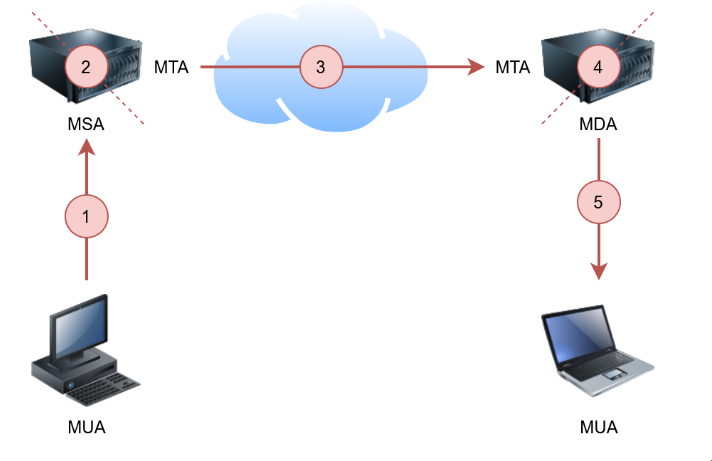
\includegraphics[width=1\textwidth]{SMTP.jpg}
\caption{SMTP}
\end{figure}

La figura muestra los siguientes cinco pasos que un email necesita pasar para llegar 
al receptor:

\begin{enumerate}
  \item Un Mail User Agent (MUA), o simplemente un cliente de email, que tiene un 
    mensaje de email a enviar. El MUA se conecta a un Mail Submission Agent (MSA)
    para mandar el mensaje.
  \item El Mail Submission Agent (MSA) recibe el mensaje, checa si hay algún error antes 
    de transferirlo al Mail Transfer Agent (MTA), comunmente hosteado en el mismo servidor.
  \item El Mail Transmission Agent (MTA) del emisor manda el mensaje email al Mail Transfer 
    Agent (MTA) del receptor. El MTA también puede actuar como un Mail Submission Agent (MSA).
  \item Una configuración típica tendría al Mail Transfer Agent funcionando también como el Mail 
    Delivery Agent (MDA).
  \item El receptor recolecta el mail del Mail  Delivery Agent usando su cliente de email.
\end{enumerate}
 Si los pasos suenan confusos, consideremos la siguiente analogía:
\begin{enumerate}
  \item Tú (el MUA) quiere mandar un mail.
  \item La oficina de correos (MSA) checa el mail para encontrar algún error, antes de que 
    la oficina local de correos (MTA) lo acepte.
  \item La oficina de correos loscal checa el destino del mail y lo manda a la oficina de correos
     en el país correcto.
  \item La oficina de correos (MTA) manda el mail al buzón del receptor (MDA).
  \item El receptor (MUA) checa el buzón para encontrar los mails. Notan el nuevo correo y lo toman. 
\end{enumerate}

De la misma manera en la que necesitamos seguir un protocolo para comunicarnos con un servidor
HTTP, necesitamos usar protocolos para comunicarnos con un Mail Transfer Agent (MTA) y un Mail Delivery Agent (MDA).
Los protocolos son:
\begin{enumerate}
  \item Simple Mail Transfer Protocol (SMTP).
  \item Post Office Protocol version 3 (POP3) e Internet Message Access Protocol (IMAP).
\end{enumerate}

El Simple Mail Transfer Protocol (SMTP) es usado para comunicarse con un servidor 
Mail Transfer Agent (MTA). Como SMTP usa texto claro, podemos usar un cliente Telnet 
para conectarse al servidor SMTP y actuar como un cliente de email (MUA) que manda un mensaje.\\

Los servidores SMTP escuchan en el puerto 25 por defecto. Para ver la comunicación 
básica con un servidor nos podemos conectar unsando un cliente Telnet.\\
Una vez conectados, usamos el comando $\textbf{helo hostname}$ y empezamos a escribir nuestro mail.
Después de $helo$, ecribimos $mail from:$, luego $rcpt to:$ para indicar el emisor y el receptor.
Después escribimos $data$ y escribimos el mensaje. Finalemnte picamos $Enter$ $.$ $Enter$ para mandar el correo.

\subsection{Post Office Protocol 3 (POP3)}
El Post Office Protocol version 3 (POP3) es un protocolo usado para descargar 
los mensajes email de un Mail Delivery Agent (MDA), como se muestra en la figura siguiente.
El cliente de mail se conecta al servidor POP3, se autentifica y descarga los mensajes antes de borrarlos.

\begin{figure}[h]
\centering
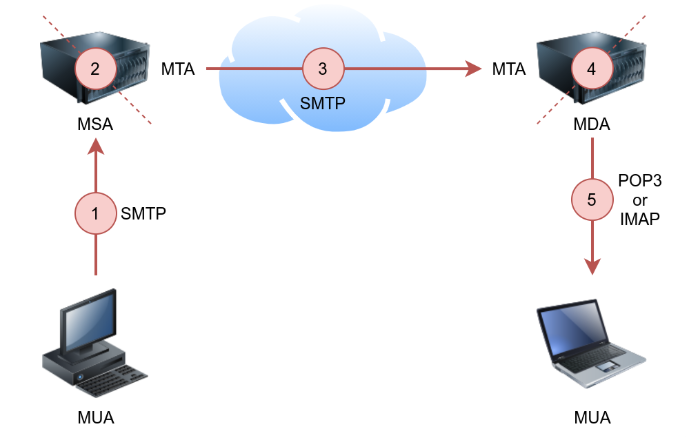
\includegraphics[width=1\textwidth]{POP3.jpg}
\caption{POP3}
\end{figure}

El ejemplo de abajo muestra cómo se ve una sesión POP3 si se usa un cliente Telnet.
Primero, el usuario se conecta al servidor POP3 cuyo puerto por defecto es el 110.
Se requiere autentificar para acceder a los mensajes de email, usando 
$\textit{USER username}$ y $\textit{PASS password}$. Usando el comando $STAT$ obtenemos 
una respuesta con la forma $\textit{+OK nn mm}$, donde $nn$ es el número de correos 
en la bandeja y $mm$ es el tamaño de la bandeja en octetos (bytes). 
El comando $LIST$ nos da una lista con los nuevos mensajes en el sevidor y $\textit{RETR 1}$
toma el primer mensaje en la lista.

\begin{figure}[h]
\centering
\includegraphics[width=1\textwidth]{POP3-Terminal.jpg}
\caption{POP3 terminal}
\end{figure}

El ejemplo de arriba muestra que los comandos son enviados en texto claro. Usar 
Telnet fue suficiente para autenticarnos y obtener el correo. Como el usuario y contraseñas
son mandados en texto claro, cualquier persona escuchando puede ver las credenciales.\\

En general, tu mail client (MUA) se conecta al servidor POP3 (MDA), se autentifica y
descarga los mensajes.\\

\subsection{Internet Message Access Protocol (IMAP)}
El Internet Access Message Protocol (IMAP) es más sofisticado que POP3. IMAP hace que sea 
posible mantener nuestros email sincrionizados en múltipes dispositivos. En otras 
palabras, si marcas un mail como leído en tu teléfono, los cambios serán salvados
en el servidor IMAP (MDA) y replicados en tu laptop cuando sincronices tu bandeja.\\

Veamos unos cuantos comandos IMAP. En la consola de abajo usamos Telnet para conectarnos
al puerto por defecto (143) del servidor IMAP y luego nos autentificamos usando 
$\textit{LOGIN username password}$. IMAP requiere que cada comando sea precedido 
por una string random para poder trackear las respuestas. 

\subsection{Resumen}


\end{document}
